\documentclass{article}
\usepackage{graphicx}
\usepackage{amsmath}
\usepackage{amsthm}
\usepackage{amsfonts}
\usepackage{mathtools}
\usepackage{algpseudocode}
\usepackage{listings}
\usepackage{graphicx}
\renewcommand{\thesubsection}{\alph{subsection}}
\begin{document}


\begin{figure}[t]

\includegraphics[width=\linewidth]{images/NTULogo}
\end{figure}
\title{CSC 401 - Advanced Topics in Algorithms}
\author{Arnav Kumar}

\maketitle

\newpage
\section{Question 1}

\subsection{$A(n) = 3A(n/4) + n^{(3/4)}$}

$A(n) = \Theta(n^{log_34})$
\begin{proof}

Inspection using Iteration method
\begin{align*}
	A(n) & = 3A(\frac{n}{4}) + n^{(3/4)} \\
	& = 9A(\frac{n}{16}) + 3(\frac{n}{4})^{3/4} + n^{3/4} \\
	& \vdots \\
	& = 3^kA(\frac{n}{4^k}) + 3^{k-1}(\frac{n}{4^{k-1}})^{3/4} + \cdots + 3(\frac{n}{4})^{3/4} + n^{3/4} \\
	& = 3^kA(1) + \sum_{i=0}^{k-1} 3^{k-1}(\frac{n}{4^{k-1}})^{3/4} \\
\intertext{Given that $A(1)$ is a constant (say $C_1$)} 
	& = 3^kC_1 + n^{3/4}\sum_{i=0}^{k-1}\frac{3^i}{4^{3i/4}} 
\intertext{$\sum_{i=0}^{k-1}3^i/(4^{3i/4})$ is a numerical constant, taking it as $C_2$}
	& = {(4^k)}^{log_34}C_1 + n^{3/4}C_2 \\
	& = n^{log_34}C_1 + n^{3/4}C_2 \\
\intertext{$n^{\log_34} = n^{0.79}$, $n^{3/4} = n^{0.75}$}
\intertext{Therefore $n^{\log_34}$ is the dominating term and,}
	A(n) & = \Theta(n^{log_34}) \\
\end{align*}

Verification using Master Theorem,

\begin{align*}
	A(n) & = 3A(\frac{n}{4}) + n^{(3/4)} \\
	a & = 3, \\
	b & = 4, \text{and,} \\
	f(n) & = n^{3/4} \\
\intertext{Is f(n) = $\mathcal{O}(n^{\log_ba - \epsilon})$?}
	\log_ba & = \log_34 = 0.79
\intertext{Because, $n^{\log_34} = n^{0.79}$, therefore,}
	f(n) & = n^{3/4} = n^{0.75} \\
	& = \mathcal{O}(n^{\log_34 - \epsilon}) \\
	\text{where, }\epsilon & = 0.04 \\
\intertext {Therefore, by Case 1 of the Master Theorem,}
	A(n) & = \Theta(n^{log_34}) \\
\end{align*}

\end{proof}

\newpage
\subsection{$B(n) = B(n-2) + n\lg n$}
$B(n) = \mathcal{O}(n^2\lg n)$
\begin{proof}

\begin{align*}
B(n) & = B(n-2) + n\lg n \\
& = B(n-4) + (n-2)\lg(n-2) + n\lg n \\
& \vdots \\
& = B(n-2k) + (n-2k+2)\lg(n-2k+2)+ \cdots \\
& + \cdots + (n-2)\lg(n-2) + n\lg n \\
\intertext{Choosing k such that $n - 2k = 1$ or $ n - 2k = 0$}
\intertext{Therefore $B(n-2k) = constant$($= c$, say)}
B(n) & = c + (n-2k+2)\lg(n-2k+2)+ \cdots + (n-2)\lg(n-2) + n\lg n \\
\intertext{$f(n) = n\lg n$, being the product of two increasing functions, $f_1(n) = n$ and $f_2 = \lg n$, is a strictly increasing function}
\intertext {We can therefore say that }
(n-2)\lg(n-2) & < (n-2)\lg n, \\
(n-4)\lg(n-4) & < (n-4)\lg n, \\
&\vdots \\
(n-2k+2)\lg(n-2k+2) & < (n-2k+2)\lg n \\
\intertext{Therefore, }
B(n) & = c + (n-2k+2)\lg(n-2k+2)+ \cdots + (n-2)\lg(n-2) + n\lg n \\
& < c + (n-2k+2)\lg n+ \cdots + (n-2)\lg n + n\lg n \\
& < c + \lg n((n-2k+2) + \dots + (n-4) + (n-2) + n) \\
& < c + \lg n(\frac{n(n-1)}{4}) \\
& < c + (\frac{n^2}{4})\lg n - (\frac{n}{4})\lg n \\
\intertext{Therefore, }
B(n) & = \mathcal{O}(n^2\lg n)
\end{align*}

\end{proof}

\newpage
\subsection{$C(n) = C(\lceil n/3 \rceil) + \lceil n/2 \rceil$}
$C(n) = \Theta(n)$
\begin{proof}

Transforming using Akra-Bazzi Theorem,
\begin{align*}
C(n) & = C(\lceil n/3 \rceil) + \lceil n/2 \rceil \\
C(n) & = \lceil n/2 \rceil + C(\lceil n/3 \rceil) && \dots (1) \\
C(n) & = \lceil n/2 \rceil + C(n/3 + h(n))\text{ where $h(n) = \lceil n/3 \rceil - n/3$} \\
\intertext{Since $0 < \lceil n/3 \rceil - n/3 < 1$} 
h(n) & = \mathcal{O}(1)
\intertext{By Akra-Bazzi Theorem, the above at (1) has the same order as,}
C'(n) & = \lceil n/2 \rceil + C'(n/3) \\
& = n/2 + (\lceil n/2 \rceil - n/2) + C'(n/3) \\
\intertext{Let's define a function $f(x) = \lceil n \rceil - n$,}
C'(n) & = n/2 + f(n/2) + C'(n/3) \\
& = n/2 + n/6 + f(n/2) + f(n/6) + C(n/9) \\
& \vdots\\
& = \frac{n}{2}(1 + \frac{1}{3} + \frac{1}{9} + \dots + \frac{1}{3^k}) \\ 
& + f(\frac{n}{2}) + f(\frac{n}{6}) + \dots + f(\frac{n}{2*3^k}) \\
& + C'(n/3^k) \dots\text{where k is such that $\frac{n}{3^k}$ is a small fraction}
\intertext{Now let,}
a & = 1 + \frac{1}{3} + \frac{1}{9} + \dots + \frac{1}{3^k} \text{ and,} \\
b & = f(\frac{n}{2}) + f(\frac{n}{6}) + \dots + f(\frac{n}{2*3^k}) \\
\intertext{Also, we know that for small constants,}
\intertext{$C'(n)$ will have constant(say, $= X_3$), O(1) values,}
\intertext{Therefore,}
C'(n) & = \frac{n}{2}a + b + X_3
\intertext{Examining the term a,}
\intertext{We know from the theory of geometric progressions that,}
\sum_{i=0}^n cr^i & = \frac{c(1-r^{n+1})}{1-r} \\
a & = 1 + \frac{1}{3} + \frac{1}{9} + \dots + \frac{1}{3^k} \\
\intertext{Therefore, for us, $c = 1$, $r = \frac{1}{3}$ and $n = k-1$}
a & = 1 * (\frac{1 - \frac{1}{3}^k}{1 - \frac{1}{3}}) \\
& = \text{a numerical constant ($= X_1$, say)} \\
\intertext{Now, examining the term b,}
\intertext{Since $0\leq f(x) < 1$ for any x,}
b & = f(\frac{n}{2}) + f(\frac{n}{6}) + \dots + f(\frac{n}{2*3^k}) \\
max(b) & < 1 + 1 + \dots + 1 \\
& = \log_3n \\
& = \frac{\lg n}{\lg 3} \text{ and,} \\
min(b) & = 0 + 0 + \dots + 0 \\
& = 0\\
\intertext{Therefore, }
C'(n) & = \frac{n}{2}X_1 + b + X_3 \\
& < \frac{n}{2}X_1 + \frac{\lg n}{\lg 3} + X_3 \\
\intertext {Hence,}
C'(n) & = \mathcal{O}(n) && \dots (2) \\ 
\intertext{Also, }
C'(n) & = \frac{n}{2}X_1 + b + X_3 \\
& \geq \frac{n}{2}X_1 + 0 + X_3 \\
\intertext {Hence,}
C'(n) & = \Omega(n) && \dots (3) \\
\intertext {Thus, from (2) and (3) we can conclude,}
C'(n) & = \Theta(n)
\end{align*}

\end{proof}


\newpage
\section{Question 2}
\subsection{Farthermost pair of vertices of a convex polygon}
We shall use a slight modification of the rotating-callipers algorithm to find our answer. We will iteratively find all the anti-podal points of the polygon. A pair of anti-podal points is defined a pair of points through which two parallel tangents can be drawn to the polygon each of which does not intersect any other edge of the polygon. We can generate all the antipodal points by first determining one pair and then rotating the tangents minimally along the sides of the polygon about one of the points of this anti-podal pair till they pass another set of antipodal points. In our algorithm, we can find our first anti-podal pair as the pair of points, first of which has the minimum y co-ordinate and the other the maximum y co-ordinate amongst the set of vertices of the polygon. We stop iterating when the total angle by which we have rotated the parallel lines becomes $\geq \pi$ because at this stage, we are back at the first anti-podal pair and each of the tangents will now iterate over points that have been iterated over by the other tangent. Let's assume two methods $angle(line_a, line_b)$ that returns the angle between lines $line_a$ and $line_b$ and $distance(point_a, point_b)$ that returns the distance between points $point_a$ and $point_b$. The anti-podal pair with the maximum distance between them is our required pair. If there are many such pairs, we return the first one to be found. 
\newline Here is the pseudo-code:
\newline
\begin{algorithmic}
\State $n \gets $\text{number of vertices}
\State $p_1 \gets $ \text{point with minimum y-co-ordinate}
\State $p_2 \dots p_n\gets $ \text{points sorted CCW according to polar angle from $p_1$\dots(1)}
\State $p_a \gets p_1 $
\State $p_b \gets $\text{point with maximum y-co-ordinate}
\State $angleRotated \gets 0 $
\State $maxDistance \gets distance(p_a, p_b)$
\State $furthermostPair \gets (p_a, p_b) $
\State $supportingLine_a \gets $ \text{horizontal vector passing thro' $p_a$ towards +ve X axis}
\State $supportingLine_b \gets $ \text{horizontal vector passing thro' $p_b$ towards -ve X axis}
\While {$angleRotated < \pi$}
	\State $edge_a \gets edge(p_a, p_{a+1})$\text{(This index wraps around. $p_{n+1} = p_1$)}
	\State $edge_b \gets edge(p_b, p_{b+1})$
	\State $angle_a \gets angle(supportingLine_a, edge_a)$
	\State $angle_b \gets angle(supportingLine_b, edge_b)$
	\If {$angle_a < angle_b$} 
		\If{$distance(p_{a+1}, p_b) > maxDistance$}
			\State $maxDistance \gets distance(p_{a+1}, p_b)$
			\State $furthermostPair \gets (p_{a+1}, p_b) $
		\EndIf
		\State $p_a \gets p_{a+1} $
	\ElsIf {$angle_b < angle_a$}
		\If{$distance(p_a, p_{b+1}) > maxDistance$}
			\State $maxDistance \gets distance(p_a, p_{b+1})$
			\State $furthermostPair \gets (p_a, p_{b+1}) $
		\EndIf
		\State $p_b \gets p_{b+1} $
	\Else \text{ (i.e. $angle_a = angle_b$) }
		\If{$distance(p_{a+1}, p_b) > maxDistance$}
			\State $maxDistance \gets distance(p_{a+1}, p_b)$
			\State $furthermostPair \gets (p_{a+1}, p_b) $
		\ElsIf{$distance(p_a, p_{b+1}) > maxDistance$}
			\State $maxDistance \gets distance(p_a, p_{b+1})$
			\State $furthermostPair \gets (p_a, p_{b+1}) $
		\ElsIf{$distance(p_{a+1}, p_{b+1}) > maxDistance$}
			\State $maxDistance \gets distance(p_{a+1}, p_{b+1})$
			\State $furthermostPair \gets (p_{a+1}, p_{b+1}) $
		\EndIf
		\State $p_a \gets p_{a+1} $ 
		\State $p_b \gets p_{b+1} $ \text{(This indices wrap around. $p_{n+1} = p_1$)}	
	\EndIf
	\State $angleRotated \gets angleRotated + min(angle_a, angle_b)$
\EndWhile
\State \Return $furthermostPair$
\end{algorithmic}

This algorithm works in $\mathcal{O}(n \lg n) time$. Let's analyze why. There are two main tasks in this algorithm:
\begin{itemize}
  \item Sorting vertices in CCW order from $p_1$
  \item Iterating through the vertices optimally to determine the pair furthest apart
\end{itemize}
We know that sorting vertices in CCW order from $p_1$ takes $\mathcal{O}(n \lg n)$ time.
\newline 
Inspecting the above algorithm, we see that we by since $angleRotated$ starts from 0 and ends at $\pi$, we can conclude that the two point variables, $p_a$ and $p_b$ iterate over every point at most once (except for the initial anti-podal pair which will also be the last pair we inspect before terminating). Therefore, the number of iterations is $\mathcal{O}(n)$.
\newline
Therefore the total running time of the algorithm $= \mathcal{O}(n \lg n) + \mathcal{O}(n) = \mathcal{O}(n \lg n)$

\newpage
\subsection{Checking if two convex hulls intersect}

Two convex hulls intersect if any one of the vertices of the first one lies strictly inside the other one. To do this, we first need to find which of the polygons is on the right of the other. We can do this by calculating their centroid (avg. of the x co-ordinates, avg. of the y co-ordinates). For the purposes of the pseudocode, let's assume the hull with m vertices is on the right. For each vertex for the left hull, we see if it lies inside the right hull. To see if a point lies inside a polygon, we draw a horizontal line from the vertex to just outside the right hull. We count the number of edges of the right hull this horizontal intersects. This will be either 1 or 2 because both are convex hulls. If it is $ = 2$, then the vertex is outside the right hull, otherwise it's inside. Here is the pseudo code.
\newline
\begin{algorithmic}
\Function {checkPolygonIntersection}{$ConvexHull$ $A$, $ConvexHull$ $B$}
	\State $P \gets  $ \text{convex hull to the left.}
	\State $Q \gets  $ \text{convex hull to the right.}
	\State $p_{1 \dots n} \gets  $ \text{points on $P$}
	\State $q_{1 \dots m} \gets  $ \text{points on $Q$}
	\State $rightmostX \gets ${the X co-ordinate of the point on $Q$ with the maximum X co-ordinate}
	\ForAll{$p$ in $p_{1 \dots n}$}
		\If{$isPointInPolygon(Q, p, rightmostX)$}
			\State \Return $true$
		\EndIf
	\EndFor 
	\State \Return $false$ \Comment {None of the points in P are inside Q} 
\EndFunction
\end{algorithmic}
\begin{algorithmic}
\Function {isPointInPolygon}{$Polygon$ $Q$, $Point$ $p$, $double$ $maxCoordiante$}
	\text {$maxCoordiante$ is the X co-ordinate of the point in Q} \\
	\text {which has the max X Co-ordinate (right most point)} \\
	\State $horizontal = LineSegment(p, Point(maxCoordiante + 1, p_y)$
	\Comment {making sure that the end of $horizontal$ is to the right of Q}
	\State $q_{1 \dots m} \gets  $ \text{points on $Q$}
	\State $count \gets 0$
	\ForAll{$q_i$ in $q_{1 \dots n}$}
		\State $edge = LineSegment (q_i, q_{i+1})$ \Comment {indices wrap around, $q_{m+1} = q_1$}
		\If{$isIntersecting(horizontal, edge)$}
			\State $count \gets count+1$
		\EndIf
	\EndFor
	\If{$count == 2$}
		\State \Return $false$
	\Else
		\State \Return $true$
	\EndIf
\EndFunction
\end{algorithmic}
\begin{algorithmic}
\Function {isPointInPolygon}{$LineSegment$ $L_1$, $LineSegment$ $L_2$}
	\State $p_1 = (x_1, y_1) \gets $ \text{starting point of $LineSegment$ $L_1$}
	\State $p_2 = (x_2, y_3) \gets $ \text{ending point of $LineSegment$ $L_1$}
	\State $p_3 = (x_3, y_3) \gets $ \text{starting point of $LineSegment$ $L_2$}
	\State $p_4 = (x_4, y_4) \gets $ \text{ending point of $LineSegment$ $L_1$}
	\If {$\lnot [(x_2 \geq x_3) \land (x_4 \geq x_1)] \land [(y_2 \geq y_3) \land (y4 \geq y1)]$}
		\State \Return $false$ \Comment{If bounding boxes don't intersect, lines can't either}
	\EndIf
	\State $ Vector$ $v1 = (p_2 - p_1)$
	\State $ Vector$ $v2 = (p_3 - p_1)$
	\State $ Vector$ $v3 = (p_4 - p_1)$
	\State $ product_1 \gets v2$ x $v1$
	\State $ product_2 \gets v3$ x $v1$
	\If {$product_1$ x $product_2 \geq 0$} \\
		\Comment{If $product_1$ x $product_2 = 0$, one (or both) $p_3$ and $p_4$ is collinear with $p_1$ and $p2$} \\
		\Comment{If $product_1$ x $product_2 > 0$, both $product_1$ and $product_2$ have the same sign, and thus the points fail the straddle test}
		\State \Return $false$
	\EndIf \\
	\text {changing the reference points (swapping roles) and doing the test again}\\
	\State $v1 \gets (p_3 - p_4)$
	\State $v2 \gets (p_1 - p_3)$
	\State $v3 \gets (p_2 - p_3)$
	\State $ product_1 \gets v2$ x $v1$
	\State $ product_2 \gets v3$ x $v1$
	\If {$product_1$ x $product_2 \geq 0$} \\
		\Comment{If $product_1$ x $product_2 = 0$, one (or both) $p_3$ and $p_4$ is collinear with $p_1$ and $p2$} \\
		\Comment{If $product_1$ x $product_2 > 0$, both $product_1$ and $product_2$ have the same sign, and thus the points fail the straddle test}
		\State \Return $false$
	\EndIf
	\State \Return $true$ \Comment{the points passed the rejection test and the two straddle tests, therefore they are strictly intersecting}
\EndFunction
\end{algorithmic}
This algorithm works in $\Theta(mn) time$. Let's analyze why. These are main tasks in this algorithm:
\begin{itemize}
  \item Finding which hull is to the right. ($\Theta(n+m)$)
  \item Finding the right-most point of the right hull. ($\Theta(m)$)
  \item Iterating through the vertices of the left hull and seeing if the vertex lies inside the the right hull
\end{itemize}

Inspecting the above algorithm, we see that to find if a point is lying inside a polygon of m sides, takes $\Theta (m)$ time because we iterate over all it's $m$ edges once. We do this for each of the $n$ vertices of the left hull, taking $\Theta (m)$ each time, totally taking $n*\Theta(m) = \Theta(mn)$ time.
\newline
Therefore the total running time of the algorithm $= \Theta(n+m) + \Theta(m) + \Theta(mn)$ \newline $= \Theta(mn)$

\newpage
\subsection{Nearest pair of vertices of two convex hulls}

We shall use a slight modification of the rotating-callipers algorithm to find our answer. We will iteratively find all the anti-podal points between the polygons. A pair of anti-podal points between two convex polygons is defined a pair of points (one from each polygon) through which a pair of anti-parallel tangents can be drawn to the respective polygons which does not intersect any other edge of that polygon. We can generate all the antipodal points by first determining one pair and then rotating the tangents minimally along the sides of the polygon till they pass another set of antipodal points. In our algorithm, we can find our first anti-podal pair as the pair of points, first of which has the minimum y co-ordinate amongst the points of the first hull and the other the maximum y co-ordinate amongst the set of points in the other hull. We stop iterating when the total angle by which the tangents have been rotated $\geq 2\pi$ because at this stage, all points of both the convex hulls have been iterated over by the respective turning tangent. Let's assume two methods $angle(line_a, line_b)$ that returns the angle between lines $line_a$ and $line_b$ and $distance(point_a, point_b)$ that returns the distance between points $point_a$ and $point_b$. The anti-podal pair with the minimum distance between them is our required pair. If there are many such pairs, we return the first one to be found.
\newline 
Here is the pseudo-code:
\newline

\begin{algorithmic}
\State $n \gets $\text{number of vertices in $P$}
\State $m \gets $\text{number of vertices in $Q$}
\State $p_1 \gets $ \text{point in $P$ with minimum y-co-ordinate}
\State $p_2 \dots p_n\gets $ \text{points sorted CCW according to polar angle from $p_1$}
\State $q_1 \gets $ \text{point in $Q$ with maximum y-co-ordinate}
\State $q_2 \dots q_n\gets $ \text{points sorted CCW according to polar angle from $q_1$}

\State $p_a \gets p_1 $
\State $q_b \gets q_1 $
\State $angleRotated \gets 0 $
\State $minDistance \gets distance(p_a, q_b)$
\State $nearestPair \gets (p_a, q_b) $
\State $supportingLine_a \gets $ \text{horizontal vector passing thro' $p_a$ towards +ve X axis}
\State $supportingLine_b \gets $ \text{horizontal vector passing thro' $q_b$ towards -ve X axis}
\While {$angleRotated < 2\pi$}
	\State $edge_a \gets edge(p_a, p_{a+1})$\text{(This index wraps around. $p_{n+1} = p_1$)}
	\State $edge_b \gets edge(q_b, q_{b+1})$\text{(This index wraps around. $q_{m+1} = q_1$)}
	\State $angle_a \gets angle(supportingLine_a, edge_a)$
	\State $angle_b \gets angle(supportingLine_b, edge_b)$
	\If {$angle_a < angle_b$} 
		\If{$distance(p_{a+1}, q_b) < minDistance$}
			\State $minDistance\gets distance(p_{a+1}, q_b)$
			\State $nearestPair \gets (p_{a+1}, q_b) $
		\EndIf
		\State $p_a \gets p_{a+1} $
	\ElsIf {$angle_b < angle_a$}
		\If{$distance(p_a, q_{b+1}) < minDistance $}
			\State $minDistance \gets distance(p_a, q_{b+1})$
			\State $nearestPair \gets (p_a, q_{b+1}) $
		\EndIf
		\State $p_b \gets q_{b+1} $
	\Else \text{ (i.e. $angle_a = angle_b$) }
		\If{$distance(p_{a+1}, q_b) < minDistance$}
			\State $minDistance \gets distance(p_{a+1}, q_b)$
			\State $nearestPair \gets (p_{a+1}, q_b) $
		\ElsIf{$distance(p_a, p_{b+1}) < minDistance$}
			\State $minDistance \gets distance(p_a, q_{b+1})$
			\State $nearestPair \gets (p_a, q_{b+1}) $
		\ElsIf{$distance(p_{a+1}, p_{b+1}) < minDistance$}
			\State $minDistance \gets distance(p_{a+1}, q_{b+1})$
			\State $nearestPair \gets (p_{a+1}, q_{b+1}) $
		\EndIf
		\State $p_a \gets p_{a+1} $ 
		\State $q_b \gets q_{b+1} $
	\EndIf
	\State $angleRotated \gets angleRotated + min(angle_a, angle_b)$
\EndWhile
\State \Return $nearestPair$
\end{algorithmic}

This algorithm works in $\mathcal{O}(n \lg n) time$. Let's analyze why. There are two main tasks in this algorithm:
\begin{itemize}
  \item Sorting vertices of P in CCW order from $p_1$. $\mathcal{O}(n \lg n)$
  \item Sorting vertices of Q in CCW order from $q_1$. $\mathcal{O}(m \lg m)$  
  \item Iterating through the vertices optimally to determine the nearest
\end{itemize}
Inspecting the above algorithm, we see that we by since $angleRotated$ starts from 0 and ends at $2\pi$, we can conclude that the two point variables, $p_a$ and $q_b$ iterate over each vertex of their respective polygons at most once. Therefore, the number of iterations is $\mathcal{O}(n+m)$.
\newline
Therefore the total running time of the algorithm $= \mathcal{O}(n \lg n) + \mathcal{O}(m \lg m) + \mathcal{O}(n+m) = \mathcal{O}(n \lg n)$ (for asymptotic upper bound)

\newpage
\section{Question 3}
\subsection{}
\begin{lstlisting}
int fib1(n)
{
	if(n==0||n==1) 
		return Soln[n];
	Soln[n-1] = fib1(n-1);
	If (Soln[n-2] == infinity) 
		Soln[n-2] = fib(n-2); 
	Soln[n]= Soln[n-1]+Soln[n-2];
	return Soln[n];
}
\end{lstlisting}

Let T(n) be the time required to compute fib1(n). \\
Observations : \\
If n$\geq 2$, the recursive call fib1(n-1) is called. That in turn computes Soln[n-2], so Soln[n-2] will never be $\infty$ and the statement Soln[n-2] = fib (n-2) is never executed and can be ignored for our calculation.\\

Therefore, 
\begin{align*}
T(0) & = \Theta(1) \\
T(1) & = \Theta(1) \\
T(n) & = T(n-1) + \Theta(1) \\
& = T(n-2) + \Theta(1) + \Theta(1) \\
& \vdots \\
& = T(n-k) + k\Theta(1) \\
\intertext{taking n = k,}
& = T(0) + n\Theta(1) \\
& = \Theta(n) \\
T(n) & = \Theta(n)\\
\end{align*}

\textbf{Space complexity} is $\mathcal{O}(n)$ because intermediate values are stored in an array of size n.

\textbf{Correctness} : This algorithm first recursively calculates the value of fib1(n-1) which leads to a call trace which results in the calculation and storage of all the Soln[i] values from 2 to n-1. Then the other condition, if $(Soln == \infty)$ never being true. Each Soln[i] value has been calculated and is correct because it = sum of Soln[i-1] and Soln[i-2].

\newpage
\subsection{}
\begin{lstlisting}
int fib2(n)
{
	if(n==0||n==1) 
		return Soln[n];
	Soln[n-2] = fib2(n-2); 
	Soln[n-1] = fib2(n-1);
	return (Soln[n-1]+Soln[n-2]); 
}
\end{lstlisting}

Let T(n) be the time required to compute fib2(n). \\
Observations : \\
\begin{align*}
T(0) & = \Theta(1) \\
T(1) & = \Theta(1) \\
T(n) & = T(n-1) + T(n-2) + 1 \\
\intertext{Here let the time taken for all the arithmetic operations in the function be 1 unit} \\
\intertext{Now, by substitution, no polynomial function $n^c$ will balance the equation, (where c is a contstant).}
\intertext{Hence we try an exponential function. $c^n$, like $T(n) = c^n$}
T(n) & = T(n-1) + T(n-2) + 1
\intertext{This equation will be easier to work with if we eliminate the constant 1 unit. Trying, $T(n) = c^n - 1$}
T(n) & = T(n-1) + T(n-2) + 1 \\
c^n - 1 & = (c^{n-1} - 1) + (c^{n-2} - 1) + 1 \\
c^n & = c^{n-1} + c^{n-2} \\
\Rightarrow c^2 - c - 1 & = 0 \\
\Rightarrow c & = \frac{1\pm\sqrt{5}}{2} \\
\intertext {Therefore, }
T(n) & = \Theta(c^n) \\
& = \Theta((\frac{1+\sqrt{5}}{2})^n) \\
\end{align*}

\textbf{Space complexity} is $\mathcal{O}(n)$ because intermediate values are stored in an array of size n.

\textbf{Correctness} : For each fib2(n) calculation, this algorithm recursively computes and saves fib2(n-1) and fib2(n-2) and saves them in Soln[n-1] and Soln[n-2] respectively before returning their sum. So though this method is more complex than the others in the question and re-computes all the intermediate values and doesn't make full use of memorization for optimization, it is correct.

\newpage
\subsection{}
\begin{lstlisting}
int fib3(n)
{
	if (n==0||n==1) 
		return Soln[n];
	Soln[n-1] = fib3(n-1);
	Soln[n] = Soln[n-1]+Soln[n-2];
	return Soln[n];
}
\end{lstlisting}

Let T(n) be the time required to compute fib3(n). \\
Observations : \\
\begin{align*}
T(0) & = \Theta(1) \\
T(1) & = \Theta(1) \\
T(n) & = T(n-1) + \Theta(1) \\
& = T(n-2) + \Theta(1) + \Theta(1) \\
& \vdots \\
& = T(n-k) + k\Theta(1) \\
\intertext{taking n = k,}
& = T(0) + n\Theta(1) \\
& = \Theta(n) \\
T(n) & = \Theta(n)\\
\end{align*}

\textbf{Space complexity} is $\mathcal{O}(n)$ because intermediate values are stored in an array of size n.

\textbf{Correctness} : This algorithm first tries to compute the fib3(n-1) and saves that in Soln[n]. This calculation involves recursively calling fib3(n-1) till fib3(1) which is known. Thereafter all the consecutive Soln[i] values are computed = Soln[i-1] + Soln[i-2] till Soln[n-1]. After which Soln[n] = Soln[n-1] + Soln[n-2] is computed and returned. This is the correct value for fib3(n).
\newpage
\subsection{}
\begin{lstlisting}
int fib4(n)
{
	if(n==0||n==1)
		return Soln[n];
	Soln[n-1] = fib4(n-1); 
	return Soln[n-1] + Soln[n-2];
}
\end{lstlisting}

Let T(n) be the time required to compute fib4(n). \\
Observations : \\
\begin{align*}
T(0) & = \Theta(1) \\
T(1) & = \Theta(1) \\
T(n) & = T(n-1) + \Theta(1) \\
& = T(n-2) + \Theta(1) + \Theta(1) \\
& \vdots \\
& = T(n-k) + k\Theta(1) \\
\intertext{taking n = k,}
& = T(0) + n\Theta(1) \\
& = \Theta(n) \\
T(n) & = \Theta(n)\\
\end{align*}

\textbf{Space complexity} is $\mathcal{O}(n)$ because intermediate values are stored in an array of size n.

\textbf{Correctness} : This algorithm first tries to compute the fib4(n-1) and saves that in Soln[n-1]. This calculation involves recursively calling fib4(n-1) till fib4(1) which is known. Thereafter all the consecutive Soln[i] values are computed till Sol[n-1]. After which Soln[n-1] + Soln[n-2] is computed and returned. This is the correct value for fib4(n).

\newpage
\section{Question 4}
\subsection{Finding maximum flow over an arbitrary n-source m-sink network}
We transform the problem into the problem of maximizing flow in 1-source 1-sink  network by adding a super source leading to each of the n sources and a super sink to which each of the m sinks lead. If n is 1 or m is 1 then the respective super element need not be added. Each of these additional connections will have infinite capacity.

We will use a refinement of the Ford-Fulkerson algorithm called the Edmunds-Karp Algorithm which uses Breadth-First Search to choose the augmenting path with the smallest number of edges.

The data structures we need are as follows:-
\begin{itemize}
\item Capacity Matrix, G[V][V], where $V = $ number of vertices, containing the capacity of the various nodes.
\item Flow Matrix $f$[V][V] containing the status of flow in the current state of the Graph.
\item S, and T, the indices of the super-source and super-sink respectively.
\item A path between points is represented as an array containing indices of the nodes of the path. 
\end{itemize}

\begin{algorithmic}
\Function{Endmunds-Karp}{$CapacityMatrix$ $G$}
	\State \text{construct an empty flow matrix} $f$
	\While {$G$ contains a path from $s$ to $t$}
		\State $P \gets $ \text{$s - t$ path in $G$ with the minimum number of edges.}
		\State \text{Augment the flow with $P$}
		\State \text{Update $f$}
		\State \text{Update $G$}
	\EndWhile
\EndFunction
\end{algorithmic}

\textbf{Analysis}: 
\begin{itemize}
\item Adding a super source and super destination takes $\mathcal{O}(n)$ and $\mathcal{O}(m)$ time respectively because it takes $\mathcal{O}(1)$ per node connected to the source or sink. $\mathcal{O}(n) + \mathcal{O}(m)$ can be approximated to $\mathcal{O}(V)$ because $m+n \leq V$
\item Using BFS to find a path (with available capacity) from s to t with the least number of nodes. Breadth first search in a graph with V vertices and E edges takes $\mathcal{O}(V+E)$ time. Since every vertex is a part of at least one edge,  $V < E$ therefore, we can say approximate the time taken for the search is $\mathcal{O}(E)$.
\item Number of augmentations is at most V x E because the longest possible path can be of length V and in each augmentation, at least one of the E edges gets saturated. So in the worst case where the path of length V, in each iteration, one of the E edges will get saturated, so in total there will be VE augmentations. Therefore the theoretical maximum number of edges augmented is VE and the while loop runs at most VE times.
\item The max flow is calculated by iterating over the m-sinks of the initial graph and seeing the flow in each of those nodes in the transformed graph. This can be done in $\mathcal{O}(m)$ time and is approximated to $\mathcal{O}(V)$ because $m < V$.
\end{itemize}

Therefore, the complexity of the algorithm is :
\begin{align*}
 & = (VE)\mathcal{O}(E) + \mathcal{O}(V) + \mathcal{O}(V) \\
 & = \mathcal{O}(VE^2)
\end{align*}

\subsection{Checking if flow is sustainable}
We do something similar to the previous problem by defining a super-source leading to all the sources and a super sink to which all the sinks lead. After that we find the maximum from though this modified graph. If for this maximal flow, the outward flow from each original source node is $\geq$ it's production rate, the the network can sustain a flow where each source node meets it's production requirement. 

For this algorithm, the complexity can be calculated as follows. We know from the previous problem that for the maximal flow, the complexity is $\mathcal{O}(VE^2)$. The additional step in this algorithm is to check if in the maximal flow all source points have met their capacity. This can be done in $\mathcal{O}(n)$ where n is the number of sources. This can be approximated to $\mathcal{O}(V)$ because $n < V$

Therefore, the complexity of this algorithm is :
\begin{align*}
 & = \mathcal{O}(VE^2) + \mathcal{O}(V) \\
 & = \mathcal{O}(VE^2)
\end{align*}

\newpage
\subsection{Algorithm in action}
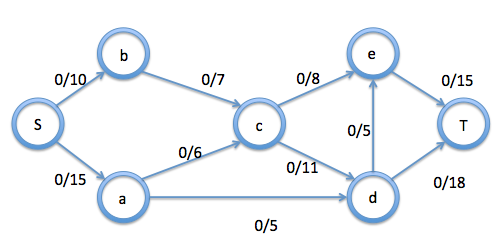
\includegraphics[width=\linewidth]{images/1}
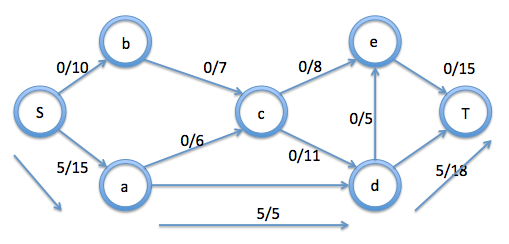
\includegraphics[width=\linewidth]{images/2}
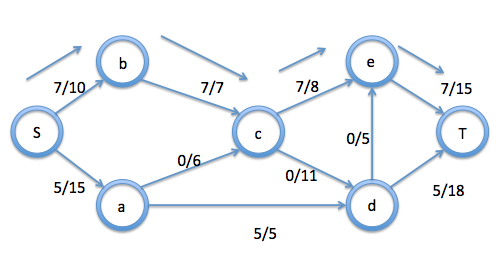
\includegraphics[width=\linewidth]{images/3}
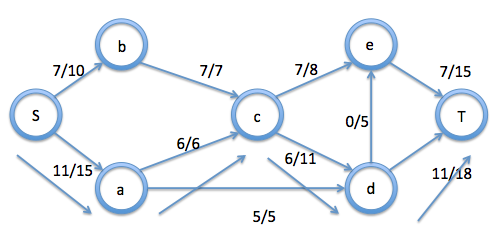
\includegraphics[width=\linewidth]{images/4}
Therefore, max flow = 18.
\begin{thebibliography}{9}

\bibitem{url1}
http://www.cs.cornell.edu/courses/cs4820/2010sp/handouts/edmondskarp.pdf

\bibitem{url3}
http://cgm.cs.mcgill.ca/~orm/rotcal.html

\bibitem{url4}
http://www.cs.uiuc.edu/class/sp07/cs473g/lectures/14-maxflowalgs.pdf

\bibitem{url2}
http://en.wikipedia.org/wiki/Edmonds–Karp\_algorithm/


\end{thebibliography}

\end{document}